\subsection{Polynomial multiplication}

\begin{frame}{Parameters}
    Our target: \texttt{hqc-128} on ARM Cortex-M4
    \begin{block}{Cryptosystem parameters}
        \begin{itemize}
            \item Maximum polynomial degree: $n = 17669$
            \item Hamming weight of sparse polynomials: $\omega = 75$
        \end{itemize}
    \end{block}
    \begin{block}{Target board}
        STM32L476RG
        \begin{itemize}
            \item 32-bit CPU
            \item 80 MHz
            \item 128 KB RAM
            \item 1 MB Flash
        \end{itemize}
        
    \end{block}
\end{frame}

\begin{frame}{Polynomial representation}
    We consider the ring of binary polynomials $\mathcal{R} = \mathds{F}_2[x] / \langle x^n+1 \rangle$
    \begin{block}{}
        We have two ways of representing binary polynomials:
        \begin{itemize}
            \item sparse: a vector of indexes, every index is a non-null coefficient
            \item dense: a vector of coefficients, every entry is a coefficient
        \end{itemize}
    \end{block}
    \begin{block}{Example}
        The polynomial $f(x) = x^{15}+x^{13}+x^8+x^6+x+1$ can be represented as:
        \begin{itemize}
            \item sparse: $[15,13,8,6,1,0]$
            \item dense: $[1,0,0,0,0,0,1,0,1,0,0,0,1,0,1,1]$
        \end{itemize}
    \end{block}
    \begin{block}{Memory usage - 32 bit architectures}
        \begin{itemize}
            \item sparse: one integer per coefficient (\emph{i.e.} 4 bytes per coefficient)
            \item dense: one bit per coefficient (\emph{i.e.}  0.25 bytes per coefficient)
        \end{itemize}
    \end{block}
\end{frame}

\begin{frame}{Shift\&Add}
    \begin{block}{}
        Multiplying a dense polynomial by $x^i$ is equivalent to a circular shift ($\clshift$) of $i$ positions to the left:
        \begin{itemize}
            \item $a(x)$ in dense representation
            \item $b(x) = [b_0, \cdots, b_{\omega-1}]$ in sparse representation
            \item Calculate $c_i(x) \gets a(x) \clshift b_i$
            \item Sum the partial results $c(x) = \sum_{i=0}^{\omega-1} c_i(x)$
        \end{itemize}
    \end{block}
    \begin{block}{Pros and cons}
        \begin{itemize}
            \item Extremely fast for $\omega \ll n$
            \item Non constant-time execution
        \end{itemize}
    \end{block}
\end{frame}

\begin{frame}{Constant time S\&A}
    Calculate all the shifts, but only sum the ones that are needed:
    \begin{block}{Monomial-Polynomial multiplication}
        Let $a(x)$ be a dense polynomial and $x^b$ a monomial, with $b = (\beta_{m-1}\beta_{m-2}\cdots\beta_0)_{\texttt{bin}}$.
        For each bit $i \in \{0, \cdots, m-1\}$, we have:
        \begin{itemize}
            \item $tmp(x) \gets a(x) \clshift i$
            \item if $\beta_i = 1$ then \texttt{mask} = $[111\cdots11]_n$, otherwise \texttt{mask} = $[000\cdots00]_n$
            \item $c(x) \gets c(x) + ((tmp(x) \wedge \texttt{mask}))$
            \begin{itemize}
                \item $\beta_i = 1$: $c(x) \gets c(x) + tmp(x)$
                \item $\beta_i = 0$: $c(x) \gets c(x) + [000\cdots00]_n$ 
            \end{itemize}
        \end{itemize}        
    \end{block}
    \begin{block}{Pros and cons}
        \begin{itemize}
            \item Constant-time execution
            \item Slower than plain S\&A
        \end{itemize} 
    \end{block}
\end{frame}

\begin{frame}{Frobenius Additive FFT}
    Based on the BIKE optimized implementation on ARM Cortex-M4~\cite{DBLP:journals/tches/ChenCK21}\\
    \begin{block}{}
        Let $a(x)$ and $b(x)$ be two dense polynomials of degree $n$ a power of 2
        \begin{itemize}
           \item Basis conversion (from monomial to novelpoly)
           \item Evaluation with the FFT
           \begin{itemize}
                \item Encode (truncated FFT)
                \item Butterflies
           \end{itemize}
           \item Pointwise multiplication
           \item Inverse FFT
           \item Basis conversion (from novelpoly to monomial)
        \end{itemize}
        Inverse operations follow the same principles of the forward ones.
    \end{block}
    Operands have fixed sizes $\rightarrow$ unroll and optimize recursive calls
\end{frame}

\begin{frame}{Basis conversion}
    Recursively split the polynomial into halves by dividing by $s_i(x)$\\
    No actual division required, just XORs:
    \begin{figure}[H]
        \begin{center}
            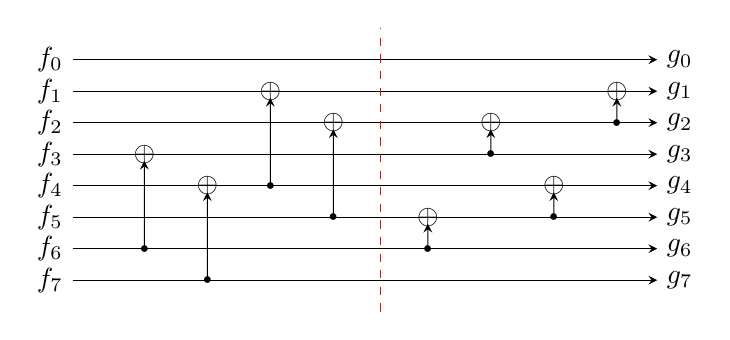
\begin{tikzpicture}[scale=0.4]
                \node (f0) at (0,7) {$f_0$};
                \node (f1) at (0,6) {$f_1$};
                \node (f2) at (0,5) {$f_2$};
                \node (f3) at (0,4) {$f_3$};
                \node (f4) at (0,3) {$f_4$};
                \node (f5) at (0,2) {$f_5$};
                \node (f6) at (0,1) {$f_6$};
                \node (f7) at (0,0) {$f_7$};
                \node (g0) at (20,7) {$g_0$};
                \node (g1) at (20,6) {$g_1$};
                \node (g2) at (20,5) {$g_2$};
                \node (g3) at (20,4) {$g_3$};
                \node (g4) at (20,3) {$g_4$};
                \node (g5) at (20,2) {$g_5$};
                \node (g6) at (20,1) {$g_6$};
                \node (g7) at (20,0) {$g_7$};
    
                \node (m1) at (3, 1)  {\tiny$\bullet$};
                \node (m2) at (5, 0)  {\tiny$\bullet$};
                \node (m3) at (7, 3)  {\tiny$\bullet$};
                \node (m4) at (9, 2)  {\tiny$\bullet$};
                \node (m5) at (12, 1) {\tiny$\bullet$};
                \node (m6) at (14, 4) {\tiny$\bullet$};
                \node (m7) at (16, 2) {\tiny$\bullet$};
                \node (m8) at (18, 5) {\tiny$\bullet$};
    
                \node (a1) at (3, 4)  {$\oplus$};
                \node (a2) at (5, 3)  {$\oplus$};
                \node (a3) at (7, 6)  {$\oplus$};
                \node (a4) at (9, 5)  {$\oplus$};
                \node (a5) at (12, 2) {$\oplus$};
                \node (a6) at (14, 5) {$\oplus$};
                \node (a7) at (16, 3) {$\oplus$};
                \node (a8) at (18, 6) {$\oplus$};
    
                \draw[-stealth] (f0) -- (g0);
                \draw[-stealth] (f1) -- (g1);
                \draw[-stealth] (f2) -- (g2);
                \draw[-stealth] (f3) -- (g3);
                \draw[-stealth] (f4) -- (g4);
                \draw[-stealth] (f5) -- (g5);
                \draw[-stealth] (f6) -- (g6);
                \draw[-stealth] (f7) -- (g7);
    
                \draw[-stealth, shorten >=-4.5pt] (m1.center) -- (a1);
                \draw[-stealth, shorten >=-4.5pt] (m2.center) -- (a2);
                \draw[-stealth, shorten >=-4.5pt] (m3.center) -- (a3);
                \draw[-stealth, shorten >=-4.5pt] (m4.center) -- (a4);
                \draw[-stealth, shorten >=-4.5pt] (m5.center) -- (a5);
                \draw[-stealth, shorten >=-4.5pt] (m6.center) -- (a6);
                \draw[-stealth, shorten >=-4.5pt] (m7.center) -- (a7);
                \draw[-stealth, shorten >=-4.5pt] (m8.center) -- (a8);
    
                \draw[dashed, color=red] (10.5, -1) -- (10.5, 8);
    
                
            \end{tikzpicture}
        \end{center}
    \end{figure}
    Also, skip the (padded) null coefficients
\end{frame}

\begin{frame}{Evaluation with the FFT}
    \begin{block}{Frobenius partition}
        Polynomial degree $2\cdot 17669 \rightarrow n = 65536$\\
        32-bit words $\rightarrow m = 32$\\
        Optimal Frobenius partition:
        \begin{equation*}
            \mathbf{S} = v_{l+m/2} + \mathbf{W}_l  = v_{27} + \mathbf{W}_{11}
        \end{equation*}
        with $l = \log_2(n/m)$
    \end{block}
    \begin{block}{Encoding}
        The first $\log_2(m)$ layers of the FFT use multipliers depending only on $m$
        \begin{itemize}
            \item Encode (truncated FFT) the first $\log_2(m)$ recursion layers
            \item \emph{Classic} butterflies for the remaining layers
        \end{itemize}
    \end{block}
\end{frame}

\begin{frame}{Encoding}
    \begin{block}{}
        The first $l_m = \log_2(m)$ layers of the FFT convert elements from
        $\mathds{F}_2^n$ to $\mathds{F}_{2^m}^{n^\prime}$.\\
        The twiggle factors can be rewritten as
        \begin{equation*}
            \begin{aligned}
                s_{l+1}(v_{l+m/2}), &\cdots, s_{l+l_m}(v_{l+m/2}) \\
                v_{m/2-1}, &\cdots, v_{m/2-l_m}
            \end{aligned}
        \end{equation*}
        so the encoding can be implemented as a linear map:
        \begin{equation*}
            g_i = \sum_{j=0}^{m-1} f_{j\cdot n^\prime +i}\cdot r_j = \begin{bmatrix} f_{0\cdot n^\prime} & f_{1\cdot n^\prime} & \cdots &f_{(m-1)\cdot n^\prime}\end{bmatrix} \cdot \begin{bmatrix}

                r_0 \\
                r_1 \\
                \vdots \\
                r_{m-1}
            \end{bmatrix}
        \end{equation*}

    \end{block}
\end{frame}

\begin{frame}{Multiplications}
    \begin{block}{Butterfly twiggle factors}
        Multiplication step: $\beta\cdot p_1(s_1(\beta))$, $\beta = (v+w) \in v_{l+m/2-i} + \mathbf{W}_{l-i}$\\
        \begin{itemize}
            \item Precompute and store all the $\beta$ values
            \item Notice that $\gamma\cdot\beta = \gamma\cdot(v+w) = \gamma\cdot v + \gamma\cdot w$
            \begin{itemize}
                \item $\gamma\cdot v$ can be computed with a binary circuit ($v$ are fixed)
                \item $\gamma\cdot w$ can be computed in a subfield to reduce the number of bits
            \end{itemize}
        \end{itemize}
    \end{block}

    \begin{block}{Pointwise multiplications}
    The resulting evaluation points are, by construction, in $\mathds{F}_{2^{32}}$.\\
    Apply Karatsuba (only once) to operate in $\mathds{F}_{2^{16}}$ and have the results
    fit in the 32-bit CPU registers.
    \end{block}
\end{frame}

\subsection{Masking}

\begin{frame}{Masking HQC}
    \begin{block}{}
    HQC operations are linear $\rightarrow$ boolean masking of the entire scheme
    \begin{equation*}
        a \mapsto \ssplit{a} = (a_1, \cdots, a_{d}) \text{ such that } \bigoplus_{i=1}^d a_i = a
    \end{equation*}
    \end{block}
    \begin{block}{Our implementation}
        More shares $\rightarrow$ slower performance, higher security\\
        We chose $d = 2$ shares:
        \begin{equation*}
            \ssplit{a} = (a \oplus x, x)
        \end{equation*}
        \begin{itemize}
            \item $a$ is the secret value
            \item $x$ is a random value (from the TRNG)
        \end{itemize}
    \end{block}
\end{frame}

\begin{frame}{Keygen}
    Mask $x$ and $y$, perform the same operations of the unmasked version
    \begin{algorithm2e}[H]
        \SetKwFunction{keygen}{\textsc{Keygen}}
        \SetKwFunction{coll}{\textsc{Collapse}}
    
        \SetKwProg{Fn}{Function}{}{}
    
        \Fn{\keygen{}}{
            $h \sample \mathcal{R}$\;
            $(x, y) \sample \mathcal{R}_\omega \times \mathcal{R}_\omega$\;
            $\ssplit{y} \gets (y+\sum \texttt{rnd}_i)$\;
            $\ssplit{s} \gets {h}\ssplit{y}$\;
            $\ssplit{s} \gets {x} + \ssplit{s}$\;
            $\kpri \gets (x, y)$\;
            $\kpub \gets (\coll{\ssplit{{h}}}, s)$\;
            \KwRet{($\kpri, \kpub$)}
        }
    \end{algorithm2e}
\end{frame}

\begin{frame}{Encryption}
    Mask $e$, $r_1$ and $r_2$, perform the same operations of the unmasked version
    \begin{algorithm2e}[H]

        \SetKwFunction{enc}{\textsc{Encrypt}}
        \SetKwFunction{coll}{\textsc{Collapse}}
    
        \SetKwProg{Fn}{Function}{}{}
        \Fn{\enc{$\kpub, {m}$}}{
            $e \sample \mathcal{R}_{\omega_e}$\;
            $(r_1,r_2) \sample \mathcal{R}_{\omega_r} \times \mathcal{R}_{\omega_r}$\;
            $\ssplit{r_1} \gets (r_1+\sum \mathtt{rnd}_i)$\;
            $\ssplit{r_2} \gets (r_2+\sum \mathtt{rnd}_i)$\;
            $\ssplit{u} \gets \ssplit{r_1} + h\ssplit{r_2}$\;
            $\ssplit{m} \gets (m+\sum \mathtt{rnd}_i) $\;
            $\ssplit{v} \gets \ssplit{m}\mathbf{G} + s \ssplit{r_2} + e $\;
            \KwRet{$(\coll{\ssplit{u}}, \coll{\ssplit{v}})$}
        }
    \end{algorithm2e}
\end{frame}

\begin{frame}{Decryption}
    \begin{columns}
        \begin{column}{0.55\textwidth}
            \begin{algorithm2e}[H]
                \SetKwFunction{dec}{\textsc{Decrypt}}
                \SetKwFunction{coll}{\textsc{Collapse}}
            
                \SetKwProg{Fn}{Function}{}{}
        
                \Fn{\dec{$\kpri, {c}$}}{
                    $\ssplit{y} \gets (y+\sum \mathtt{rnd}_i)$\;
                    $\ssplit{uy} \gets u \ssplit{y}$\;
                    $\ssplit{\bar{m}} \sample (\{0,1\}^k)^d$\;
                    $\ssplit{\bar{c}} \gets \ssplit{\bar{m}}\mathbf{G}$\; 
                    $a \gets \coll{(v ,\ssplit{\bar{c}})}$\;
                    $m \gets \text{\sc Decode}(\coll{a,\ssplit{uy}})$\;
                    \KwRet $\coll{m ,\ssplit{\bar{m}}}$\;
                }
            \end{algorithm2e}
        \end{column}
        \begin{column}{0.45\textwidth}
            \begin{block}{}
                Generate a random message $\ssplit{\bar{m}}$\\
                Encode it $\ssplit{\bar{c}} = \ssplit{\bar{m}}\mathbf{G}$\\
                Add the first half of the ciphertext\\
                Collapse it together with the second half of the ciphertext\\
                Decode the result\\
                Remove the random message
            \end{block}
        \end{column}
    \end{columns}
    \begin{block}{Linearity of the RMRS code}
        \begin{equation*}
            \textsc{Encode}(m_1 + m_2) = \textsc{Encode}(m_1) + \textsc{Encode}(m_2)
        \end{equation*}
    \end{block}
    
\end{frame}